\newif\ifrevtex
\revtextrue

\ifrevtex
    \documentclass[aps,prd,final,twocolumn,letterpaper,nofootinbib]{revtex4-1}
\else
    \documentclass[twocolumn]{article}
\fi

%\usepackage[letterpaper,hmargin=0.8in,vmargin=0.8in]{geometry}
\usepackage{graphicx}

\usepackage{amsmath,amssymb}
\usepackage{siunitx}

\usepackage{cleveref}

%\usepackage{mathpazo}
\usepackage{microtype}

\usepackage{diagbox}
\usepackage{multirow}

\usepackage{color}
%\usepackage[printwatermark]{xwatermark}
%\newwatermark[allpages,color=red!10,angle=45,scale=3,xpos=0,ypos=0]{DRAFT}

\usepackage{tikz}

\newcommand\RR{\mathbb{R}}
\DeclareMathOperator\im{im}

\newcommand{\mb}{\mathbf}

%\usepackage{tikz}
%\usetikzlibrary{arrows}
%\usetikzlibrary{angles,patterns,calc}

\newcommand\headers{
    \title{Rigiditea: web-based rigidity algorithms}
    \author{Tony Zhang and Menghua Wu}
    \date{May 17, 2017}    
    \begin{abstract}
        We present Rigiditea,
        a native client-side web-based implementation of two algorithms
        for testing generic rigidity of graphs:
        the $n$-dimensional randomized infinitesimal-rigidity-based algorithm
        and the deterministic pebble game algorithm for two-dimensional rigidity.
        For the latter, we provide a step-by-step visualization of the algorithm
        for aid in understanding the algorithm.
    \end{abstract}
}


\ifrevtex\relax\else\headers\fi
\begin{document}
\ifrevtex\headers\fi

\maketitle



% % % % % % % % % %
%    INTRODUCTION
% % % % % % % % % %

\tableofcontents

\section{Introduction}

The theory of linkages TODO TODO TODO
finds obvious applications.
For example, 

We implemented two major algorithms for generic rigidity.
The first, which works in $n$ dimensions,
considers a random embedding of the graph into $\RR^n$
and computes the number of infinitesimal degrees of freedom (dof)
as described in \cite[\S4.4.2]{gfalop}.
Infinitesimal rigidity of the random embedding always implies generic rigidity;
the converse holds with high probability.

The second algorithm is the famous \emph{pebble game algorithm},
first introduced by Jacobs and Hendrickson in 1997~\cite{jacobs97}.
Briefly, it considers TODO TOOD

To the best of our knowledge,
there do not exist convenient implementations of
either rigidity algorithm.
In particular,
we were unable to find an sort of graphical interface
for the infinitesimal algorithm,
and only found a Java applet for the pebble game \cite{stjohnapplet}.


TODO TODO

Let us outline the remainder of this paper.
In \cref{sec:arch}, we describe the structure of our web application.
We next develop the theory behind the two rigidity algorithms
in \cref{sec:pebble,sec:infrigid}
to the level of detail necessary for understanding our work.
(Notably, we introduce a correction in \cref{sec:infrigid}
to the well-known formula for the infinitesimal dof of a linkage.)
We conclude with a discussion of possible extensions to Rigiditea.

\section{Architecture}
\label{sec:arch}

blah blah blah

\subsection{Interface}

We provide an aesthetic graphical user interface (GUI)
to design and analyze linkages as 2D planar graphs.

\begin{figure}[ht]
\begin{tikzpicture}
\node at (0,0) {
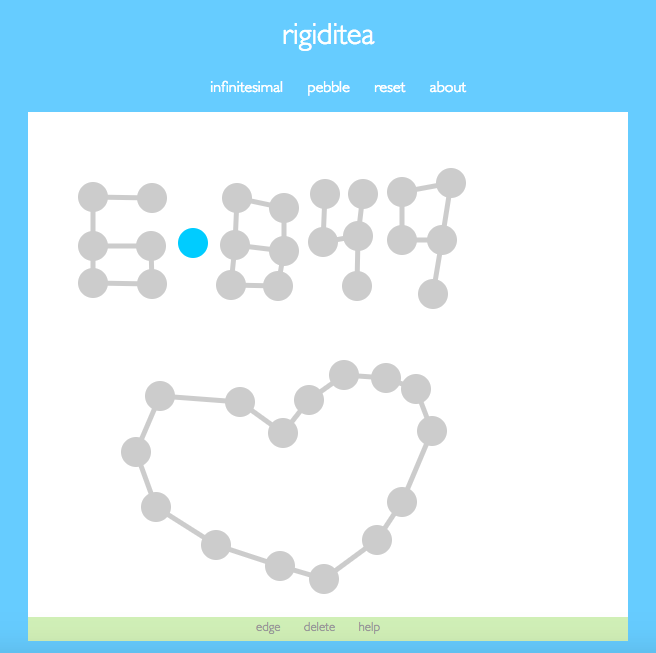
\includegraphics[scale=.3]{img/ui}
};
\draw (-3,-2.7) rectangle (3,2);
\node at (0,-1.5) {\large graph-drawing canvas};

\draw (-2,2.2) rectangle (2,2.7);
\node at (-2.5,2.45) {menu};

\draw (-1.5,-3) rectangle (1.5,-3.3);
\node at (-2.4,-3.15) {controls};
\end{tikzpicture}
\caption{High level overview of graphical user interface.
We aimed for a simple, but powerful design.}
\label{fig:ui}
\end{figure}

First, a user may click anywhere on the canvas to add a new node to the graph.
After creating nodes,
a user can control the user interface through one of two ways:
the menu bar and the control panel.
The former focuses on algorithm running and general information,
while the latter is tailored towards graph creation.
\Cref{fig:ui} points out these elements in the actual interface.
In addition to the menu and control panel,
we also provide keyboard shortcuts to streamline the user experience.
\Cref{tab:menu} enumerates the various commands available,
their functionalities, and keyboard shortcuts.

\begin{table}[ht]
\caption{Control panel items and descriptions.}
\def\arraystretch{1.5}
\begin{tabular}{c | c | p{0.5\linewidth} | c}
& item & description & key \\ \hline
\multirow{3}{.5cm}{\rotatebox{90}{menu bar items~~}}
& pebble & advances pebble algorithm one step
(one pebble exchange) & $\to$\\
& reset & resets defaults, initializes new graph, wipes canvas & r \\
& about & background information about algorithms,
web application, and further reading & a \\\hline
\multirow{3}{.5cm}{\rotatebox{90}{control panel~~}} &
edge & draws an edge between two selected vertices & e\\
& delete & deletes all selected components, including incident edges
to selected nodes & x \\
& help & provides information about graph designing interface,
including keyboard shortcuts & h \\
\end{tabular}
\label{tab:menu}
\end{table}

The GUI was created using \texttt{d3.js},
an open-source data visualization library for web applications.
We selected this library
to directly link graph data objects to SVG elements on the canvas.

\subsection{Graph representation}

Graphs were represented as custom Javascript \texttt{Graph} objects,
each with a list of \texttt{nodes}, \texttt{edges}, and specialized instance methods.
We will later introduce the \texttt{PebbleGraph} class,
which is a subclass of \texttt{Graph} with additional rigidity-related capabilities.

Each \texttt{Edge} object keeps track of its unique \texttt{id}, \texttt{source}, \texttt{target}, and \texttt{attributes},
such as current and previous color.
Of these fields, \texttt{source} and \texttt{target} are both \texttt{Node} objects,
which each possess a unique \texttt{id}, its \texttt{x} and \texttt{y} coordinates,
and a map of \texttt{attributes}.
Unique \texttt{id}s were randomly generated,
case-sensitive alphanumeric strings of 5 characters.
Figure \ref{fig:graphrep} provides a simple example.

Note that nodes are passed to \texttt{edges} by reference.
Furthermore, we use an absolute coordinate system,
based on pixels, so for convenience, each node keeps track of its own location.

\begin{figure}[ht]
\begin{verbatim}
Graph: {
   nodes: {
     Node:
       {id: a6849, x:68, y:49, attr: {fill: #CEF}},
     Node:
       {id: b6867, x:68, y:67, attr: {fill: #FCE}}},
   edges: {
     Edge:
       {source: Node, target: Node,
         attr: {stroke: #CEF}}},
         ...
   [instance methods]
}
\end{verbatim}
\caption{Sample representation of a line segment.}
\label{fig:graphrep}
\end{figure}

On top of this basic graph,
we designed another \texttt{PebbleGraph} class,
which could run iterations of the pebble algorithm
and test for infinitesimal rigidity.
\texttt{PebbleGraph} objects can be easily created
from standard \texttt{Graph} objects since
their underlying representations are the same.
However, \texttt{PebbleGraph} objects also maintain
an assignment of ``pebbles'' to edges and vertices.
Thus, once we begin running the Pebble algorithm,
we disable graph editing in the GUI and generate a mutable \texttt{PebbleGraph}
for future steps.
 
\subsection{Backend}
blah

\section{Pebble game visualization}
\label{sec:pebble}

Rigiditea primarily provides a pebble game visualization,
in which we attempt to add edges and see if they contribute
to the graph's overall rigidity.

At each phase, we randomly select an edge to ``add'' to our current set.
For four rounds, we attempt to cover the edge with four pebbles.
This is reflected in our GUI with a spectrum of blue and green,
where zero pebbles is a darker blue and four pebbles is a light yellow-green.
Pebbles can reside in both nodes and edges,
so both can be colored.
Figure \ref{fig:pebbles} demonstrates this process
for a triangle.

\begin{figure*}[t]
   \centering
   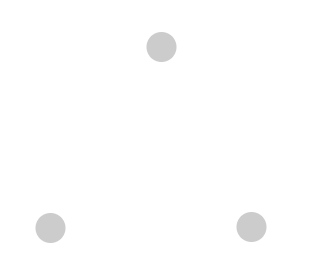
\includegraphics[width=.24\linewidth]{img/t1}
   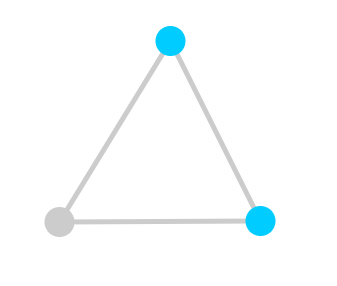
\includegraphics[width=.24\linewidth]{img/t2}
   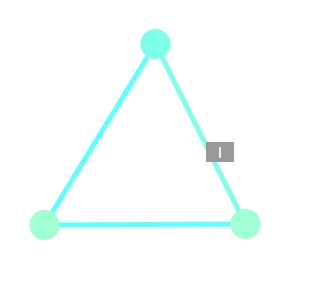
\includegraphics[width=.24\linewidth]{img/t3}
   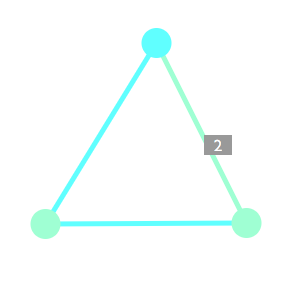
\includegraphics[width=.24\linewidth]{img/t4}
   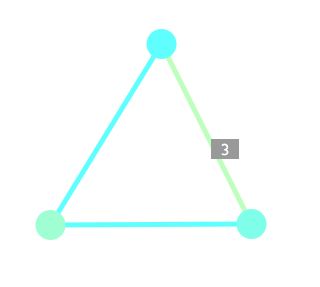
\includegraphics[width=.24\linewidth]{img/t5}
   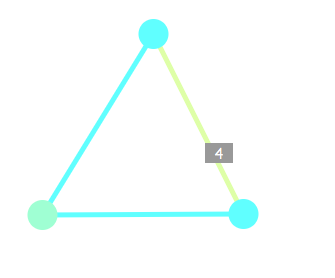
\includegraphics[width=.24\linewidth]{img/t6}
   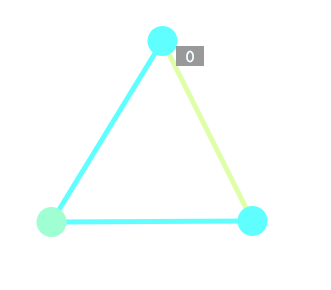
\includegraphics[width=.24\linewidth]{img/t7}
   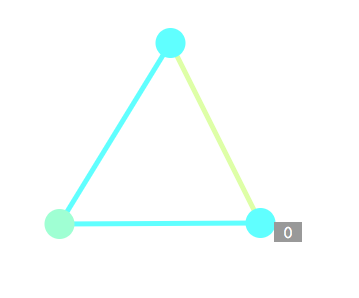
\includegraphics[width=.24\linewidth]{img/t8}
   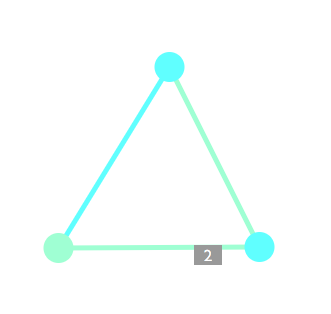
\includegraphics[width=.24\linewidth]{img/t9}
   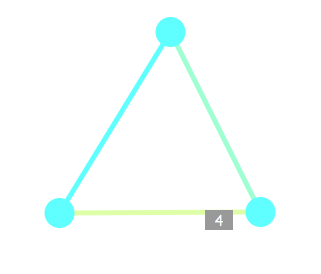
\includegraphics[width=.24\linewidth]{img/t10}
   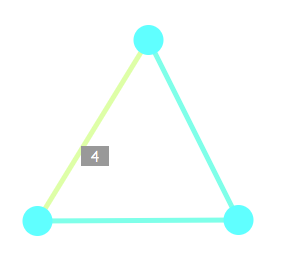
\includegraphics[width=.24\linewidth]{img/t11}
   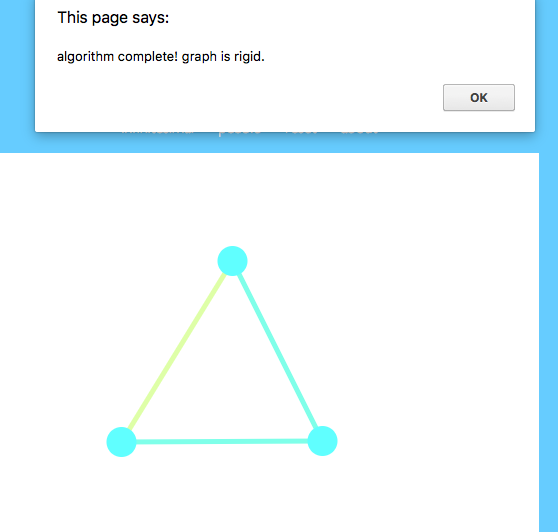
\includegraphics[width=.24\linewidth]{img/t12}
   \caption{Process of a single pebble game for a triangle.
   The labels on each edge or node show the number of pebbles on that element.
   We can see that the number of pebbles increases each time from 1 to 4,
   as the pebbles on nodes are transferred to edges.
   In the final frame, we see that the triangle is successfully identified as rigid.}
   \label{fig:pebbles}
\end{figure*}

\section{Infinitesimal rigidity}
\label{sec:infrigid}

In this section,
we outline the algorithm for determining the infinitesimal degrees of freedom
of a $d$-dimensional linkage embedding.
The algorithm is straightforwardly presented in \cite[\S4.4.2]{gfalop},
so we only provide a brief sketch.
More importantly, however,
we shall prove a correction to the formula the algorithm uses
to compute the infinitesimal degrees of freedom.

Suppose we have a graph $G = (V, E)$ of $n$ vertices and $m$ edges.
Given a $d$-dimensional embedding of the vertices,
each edge provides a linear constraint
on the allowed infinitesimal motions of $V$.
In matrix form, we can write
\begin{equation}
    R\mb v = 0
\end{equation}
for a \emph{rigidity matrix}~$R$ of shape $dn \times m$
and an infinitesimal motion $\mb v \in \RR^{dn}$,
whose components are the $d$ components
of the infinitesimal motion of each of $n$ vertices.

The space of allowed infinitesimal motions is then $\ker R$.
However, some of these motions are rigid,
corresponding to the infinitesimal generators of rigid motions in $\RR^d$,
which form a $\binom{d+1}{2}$-dimensional vector space:
the Lie algebra $\mathfrak{se}(d)$ of the \emph{special Euclidean group},
the orientation-preserving isometry group of $\RR^d$.

Once we exclude these trivial motions,
we would naively expect the subspace of nontrivial infinitesimal motions
to have dimension
\begin{equation}\label{eq:wrong-infdof}
    \dim\ker R - \binom{d+1}{2} = dn - \dim\im R - \binom{d+1}{2},
\end{equation}
as presented in \cite{gfalop}.

This formula is generally correct,
but fails badly for some elementary examples.
For instance, take $K_2$, the graph of two vertices joined by an edge.
The rigidity matrix will have rank 1,
so for sufficiently large $d$,
we expect negative degrees of freedom:
\[
    dn - 1 - \underbrace{\binom{d+1}{2}}_{\Theta(d^2)} < 0.
\]
Of course, $K_2$ should have no degrees of freedom for any~$d$,
so we're clearly overcompensating in accounting for rigid motions.

Indeed, the naive analysis above
assumed that the subspace~$M_0$ of trivial motions in $\ker R$
was $\binom{d+1}{2}$-dimensional:
that is, each nontrivial infinitesimal isometry of $\RR^d$
produced a nontrivial infintiesimal motion of our graph.
This assumption is generally false.
In our $K_2$ example,
if $d=3$, 
the infinitesimal generator
of the rotation about the single edge
produces the trivial infinitesimal motion 0
of the two vertices.

We'd like to find $\dim M_0$,
which will give the correct number of independent rigid motions
for which we need to compensate in \cref{eq:wrong-infdof}.
To this end,
consider the linear map $\phi\colon\mathfrak{se}(d) \to M_0$
that takes an infinitesimal Euclidean isometry
and gives the associated rigid motion of the linkage.

The dimension formula gives
\[
    \dim M_0 = \dim\mathfrak{se}(d) - \dim\ker\phi.
\]
The first term is the well-known dimensionality $\binom{d+1}{2}$
of rigid motions in $\RR^d$.
The second term takes more care.

By definition, $\ker\phi$ gives the infinitesimal isometries
that fix the vertices of the linkage,
Let the origin of $\RR^d$ be one of these vertices
and note that any $u\in \mathfrak{se}(d)$ fixes the origin;
therefore, $u\in\mathfrak{so}(d)$
(the Lie algebra of the group
of orientation-preserving orthogonal linear maps on $\RR^d$)
is a linear operator on $\RR^d$.

Since $u$ generates an isometry fixing all vertices of the linkage,
$u$ vanishes on all of them.
So $u$ vanishes on the lowest-dimensional flat containing all the vertices;
say this flat has dimension $k$.
Then $\ker\phi\cong\mathfrak{so}(d-k)$, which has dimension $\binom{d-k}{2}$.
(Intuitively: if a $d$-dimensional rotation fixes a $k$-dimensional subspace,
it's really a $d-k$-dimensional rotation.)

As a result, the correct formula we want is
\begin{equation}
    dn - \dim\im R - \binom{d+1}{2} + \binom{d-k}{2}.
\end{equation}
We are not aware of prior work mentioning the final correction term we derived.

Note that this algorithm immediately turns into an algorithm
for testing generic linkage rigidity in arbitrarily many dimensions $d$.
Since random embeddings are generic with high probability,
the infinitesimal dof will almost always match the generic dof.
So testing generic rigidity reduces to testing infinitesimal rigidity.


\section{Discussion}

\subsection{Comparison to existing implementation}

There currently exists another
implementation of the pebble algorithm as a Java application.
[TODO REFERENCE]

Compared to Rigiditea, this implementation
has more built-in features and is a more mature application,
but as a fully front-end web application,
Rigiditea is more accessible, easy-to-use, and pleasing to look at.
Rigiditea also offers complete flexibility in graph design,
instead of using several existing shapes for demonstration purposes.
Table \ref{tab:comp} provides an extensive comparison of the two software.
On a whole, Rigiditea is not meant to replace the existing tool,
but rather to provide a simpler tool for those casually interested
in rigidity.


\begin{table*}[ht]
\def\arraystretch{1.5}
\caption{Comparison of Rigiditea and existing Java implementation
across different features and criteria.}
\begin{tabular}{p{0.4\linewidth} | p{0.4\linewidth}}
Rigiditea & Java implementation \\ \hline
minimalist web GUI, completely front-end, can be hosted anywhere
without a backend &
Java application, requires download to run (most systems have a JVM) \\
aesthetic design, fun to play with, keyboard shortcuts convenient &
standard software developer look, though with intuitive icons
and a thorough menu\\
draw graphs completely freehand,
with simple editing tools &
select from a set of sample graphs,
which demonstrate certain concepts \\
graphs are fixed in location and scale &
graphs can be rotated and moved around point or segment \\
visualize individual steps of pebble algorithm &
visualize individual steps of pebble algorithm\\
tests for linkage rigidity & tests for linkage rigidity\\
only provides overall rigidity & finds over-braced components \\
provides tester for infinitesimal rigidity in $n$ dimensions,
independent of the pebble algorithm
& not a design goal
\end{tabular}
\label{tab:comp}
\end{table*}

\section{Extensions}

There are several extensions we may explore for our web application.

On the web interface side,
it would be convenient to scroll through the pebble algorithm's steps
in a timeline, similar to that of the existing Java implementation.
This feature could be easy to implement,
if we simply maintain a history of the \texttt{PebbleGraph} objects
and display one of them depending on the time step.
Furthermore, it would be convenient to export the resultant graph into FOLD,
as a linkage. However, we did not prioritize this goal since
linkages can be adequately visualized as planar graphs,
which are general in concept.

Algorithmically, we would also like to visualize rigid components of a linkage.
It would be ideal to color the over-braced,
under-braced, and minimally rigid components so a user
can distinguish between them.
The pebble algorithm can determine such components [TODO],
but we did not have the time to implement this element here.

Finally, we would like to extend this web application to other pebble games
such as [lee08, chubynsky07]


\section*{Acknowledgements}


\bibliography{rigiditea}{}
\bibliographystyle{plain}






\end{document}

